\section{DESARROLLO} 

\subsection{Desarrollo del Sistema}
\begin{enumerate}[1.]
	\item Pasos de desarrollo de la aplicacion
	\begin{enumerate}[a)]
	\item Paso 1: Diagrama de Clases de solución Cajero
		\begin{figure}[H]
		\begin{center}
		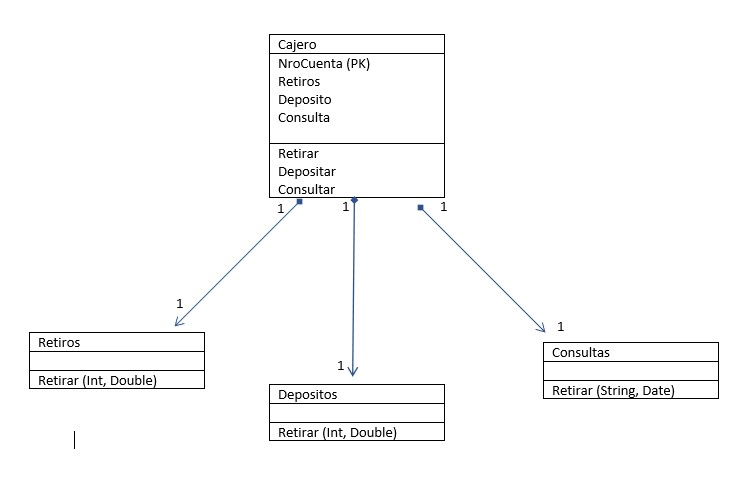
\includegraphics[width=8cm]{./Imagenes/img1}
		\end{center}
		\end{figure}
	\item Paso2: Crear un Windows form para desorrallar nuestra aplicación de escritorio:
		\begin{figure}[H]
		\begin{center}
		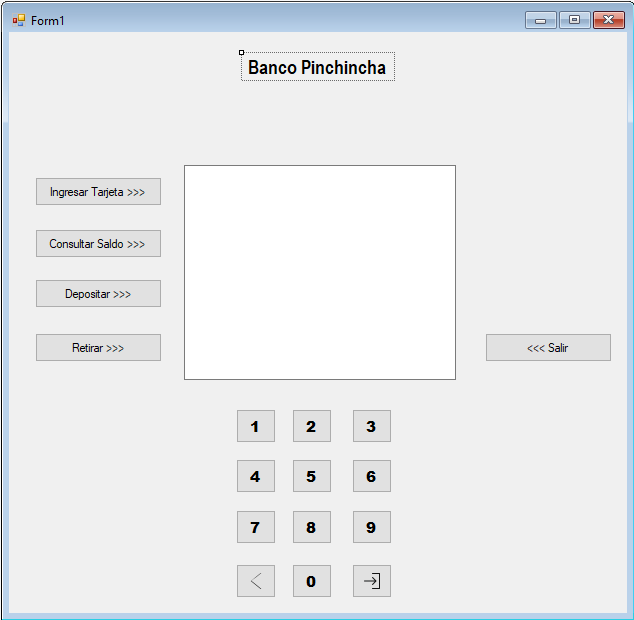
\includegraphics[width=6cm]{./Imagenes/img2}
		\end{center}
		\end{figure}
	\item Paso 3: Codificar los botones según lo planeado para nuestra aplicación, por ejemplo para esta aplicación hemos decidido 		virtualizar un cajero automático. \\
		\begin{figure}[H]
		\begin{center}
		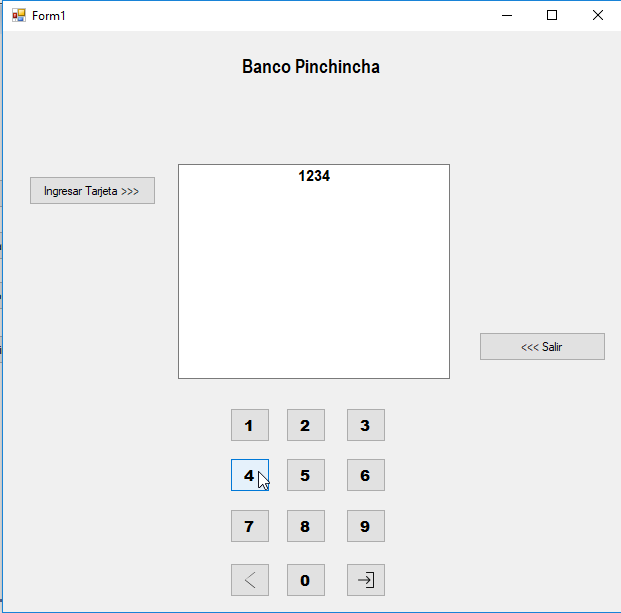
\includegraphics[width=7cm]{./Imagenes/img3}
		\end{center}
		\end{figure}
	\item Paso 4: Muestra de algo de código de los botones: 
		\begin{figure}[H]
		\begin{center}
		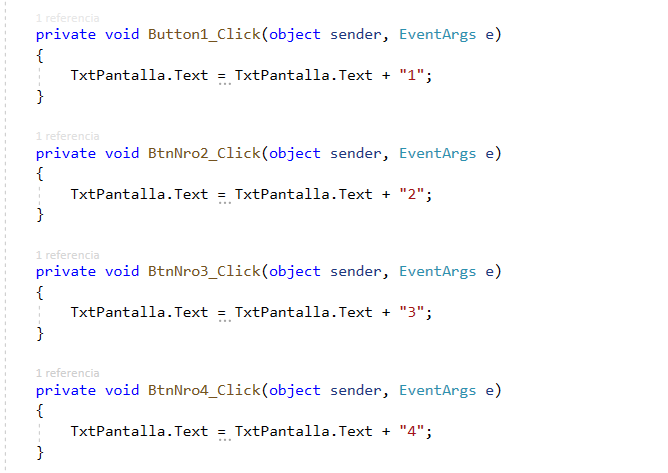
\includegraphics[width=6cm]{./Imagenes/img4}
		\end{center}
		\end{figure}
	\item Paso 5: aplicar un ORM a nuestra aplicación: aplicaremos el ORM Entity framework(define que es y para que sirve  entity framework) 
		\begin{figure}[H]
		\begin{center}
		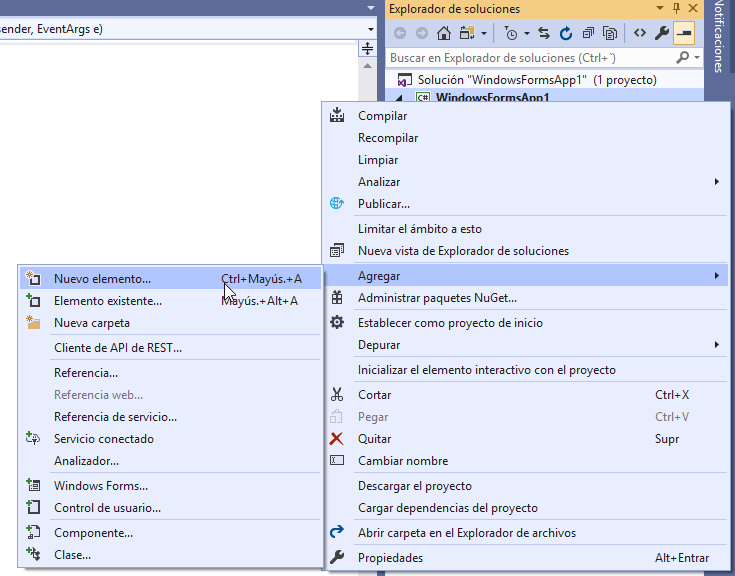
\includegraphics[width=7cm]{./Imagenes/img5}
		\end{center}
		\end{figure}
	\item Paso 6: Agregaremos el modelo ADO.NET entity data model
		\begin{figure}[H]
		\begin{center}
		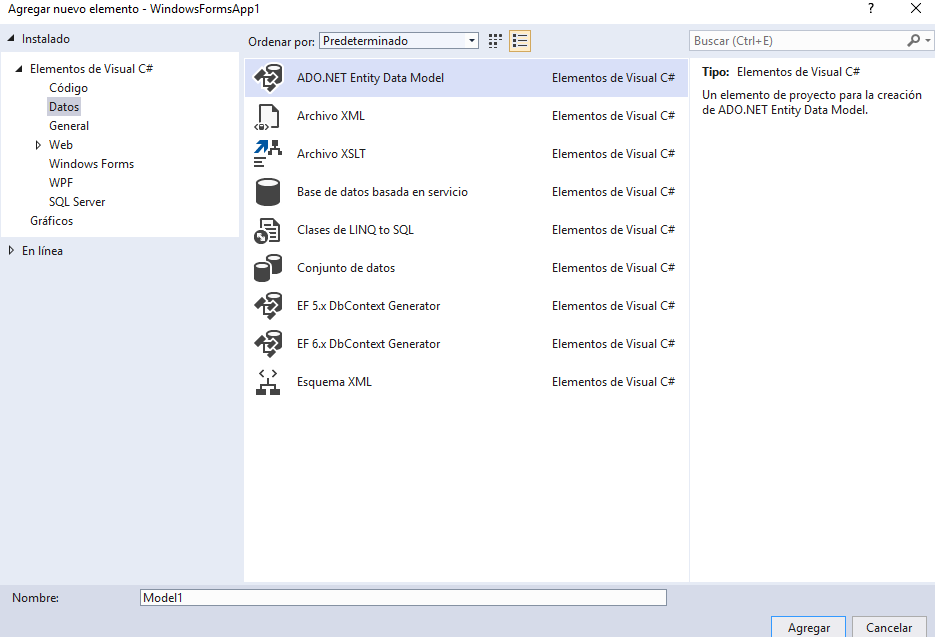
\includegraphics[width=7cm]{./Imagenes/img6}
		\end{center}
		\end{figure}
	\item Paso 7: ELuego configuraremos con la base de datos que se encuentra en Nuestro servidor SQL 
		\begin{figure}[H]
		\begin{center}
		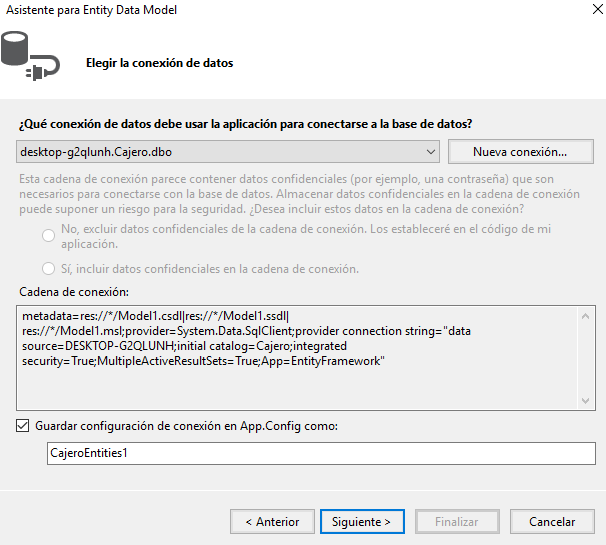
\includegraphics[width=8cm]{./Imagenes/img7}
		\end{center}
		\end{figure}
	\item Paso 8: una vez configurado podremos comprobar que ya podemos interactuar con la base de datos a través Entity Framework.
		\begin{figure}[H]
		\begin{center}
		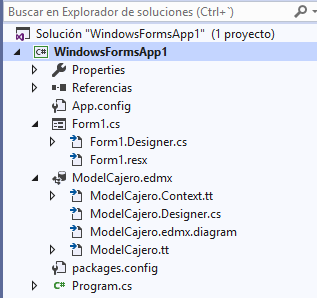
\includegraphics[width=8cm]{./Imagenes/img8}
		\end{center}
		\end{figure}
		-  Despues escribrir la siguiente consulta.
		\begin{figure}[H]
		\begin{center}
		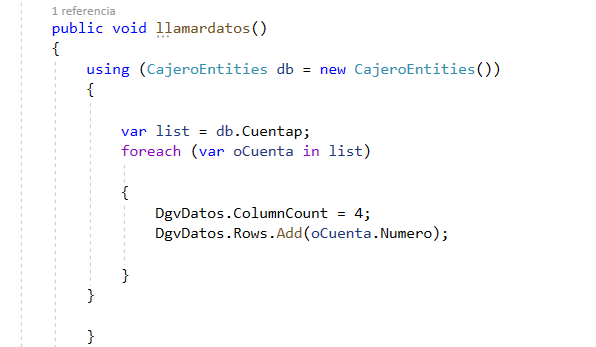
\includegraphics[width=5cm]{./Imagenes/img9}
		\end{center}
		\end{figure}
	\item Paso 9: Demostraremos el de entity framework con un Login. Para lograr esto liste los datos de Tarjeta que se encuentran en la base de datos en un DataGridView (Por motivos de 		Seguridad este DataGridView no será visible para el Usuario) con el siguiente código:
		\begin{figure}[H]
		\begin{center}
		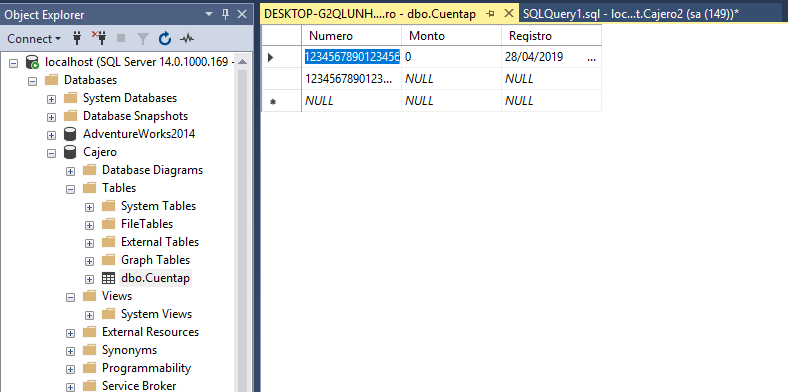
\includegraphics[width=7cm]{./Imagenes/img10}
		\end{center}
		\end{figure}
	\item Paso 10: Demostraremos el de entity framework con un Login. Para lograr esto liste los datos de Tarjeta que se encuentran en la base de datos en un DataGridView (Por motivos 			de Seguridad este DataGridView no será visible para el Usuario) con el siguiente código:
		\begin{figure}[H]
		\begin{center}
		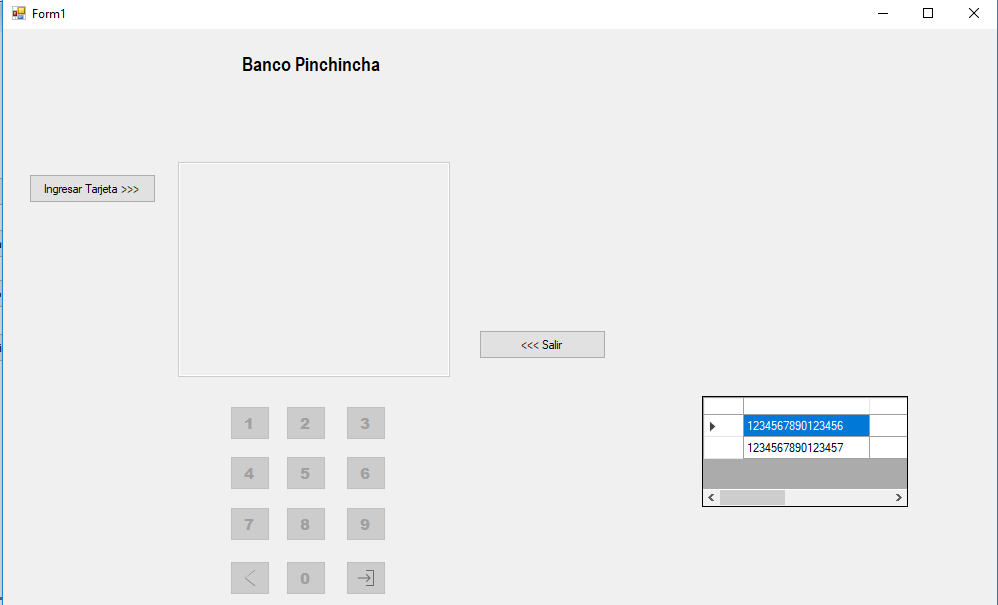
\includegraphics[width=6cm]{./Imagenes/img11}
		\end{center}
		\end{figure}
	\item Paso 11: Una vez obtenidos los datos podremos confirmar si el usuario existe o no en la base de datos:
		Codigo:
		\begin{figure}[H]
		\begin{center}
		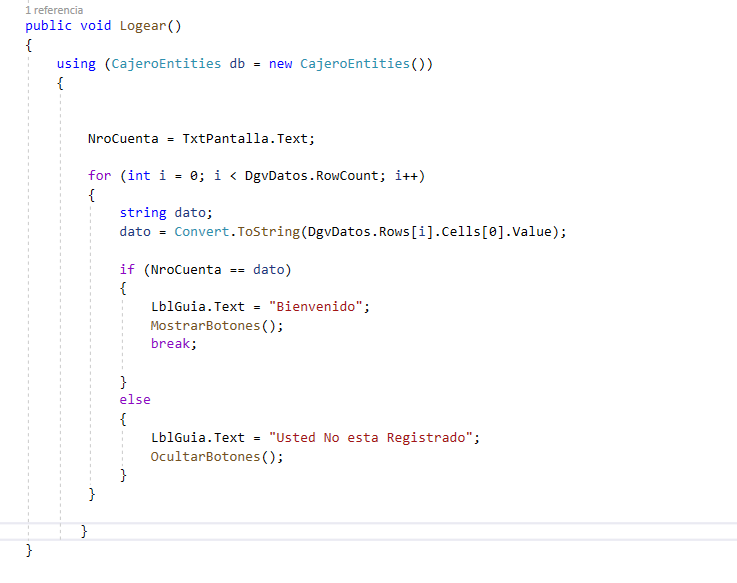
\includegraphics[width=7cm]{./Imagenes/img12}
		\end{center}
		\end{figure}
	\item Paso 12: Se muestra el formulario principal del cajero
		\begin{figure}[H]
		\begin{center}
		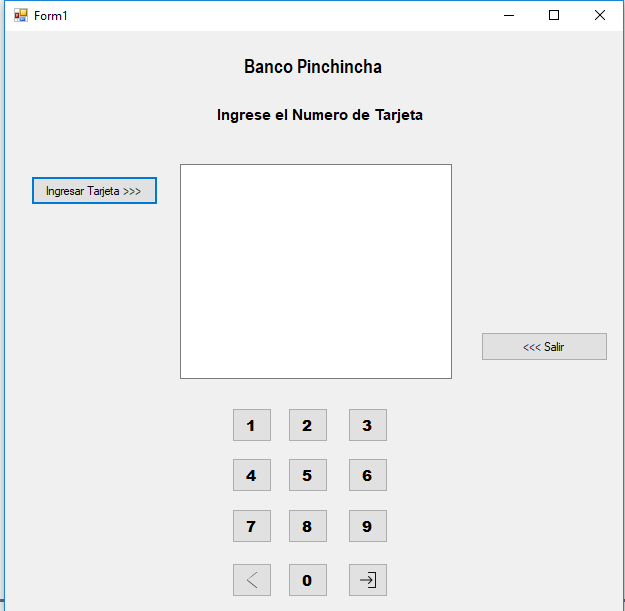
\includegraphics[width=7cm]{./Imagenes/img13}
		\end{center}
		\end{figure}
	\item Paso 13: Si existe el formulario
		\begin{figure}[H]
		\begin{center}
		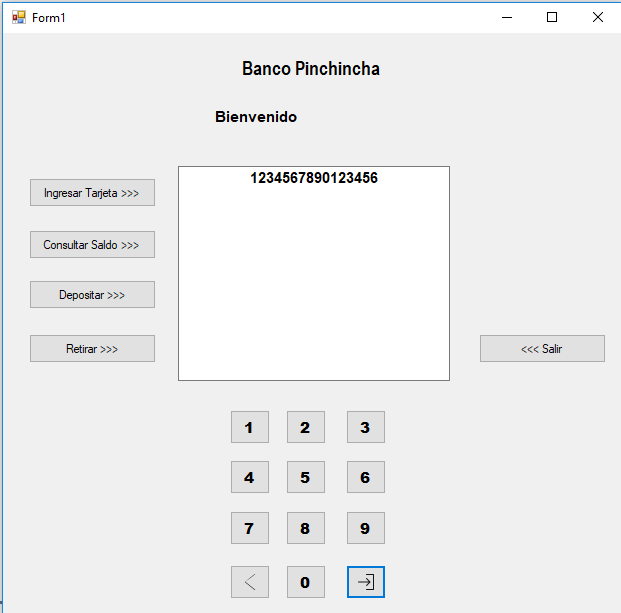
\includegraphics[width=7cm]{./Imagenes/img14}
		\end{center}
		\end{figure}
	\item Paso 14: Si en caso que no existe
		\begin{figure}[H]
		\begin{center}
		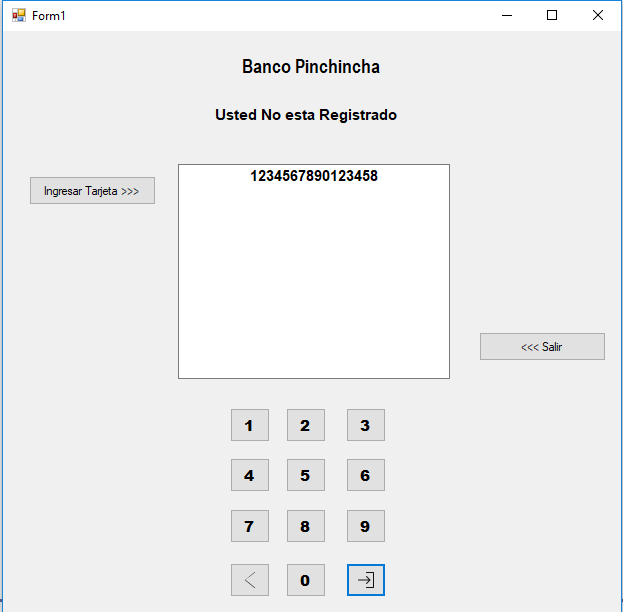
\includegraphics[width=7cm]{./Imagenes/img15}\\

		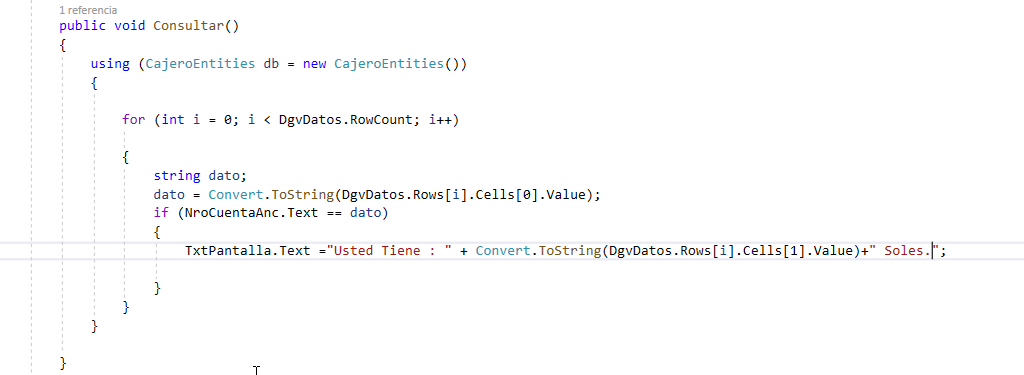
\includegraphics[width=7cm]{./Imagenes/img16}\\

		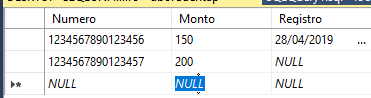
\includegraphics[width=7cm]{./Imagenes/img17}\\

		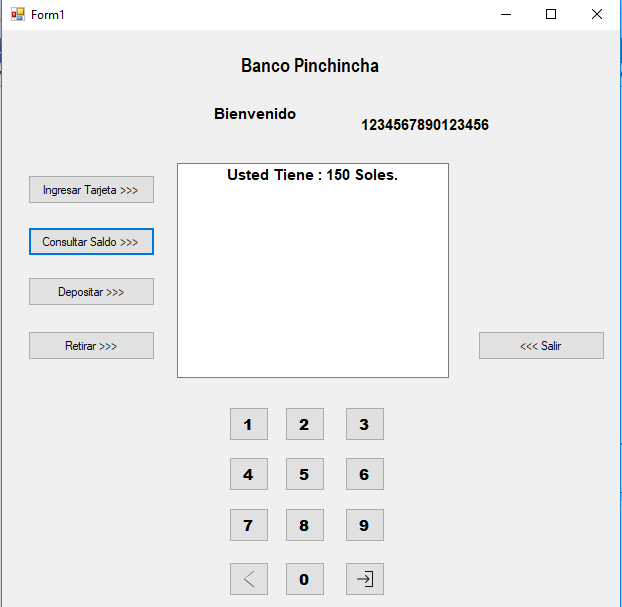
\includegraphics[width=7cm]{./Imagenes/img18}\\

		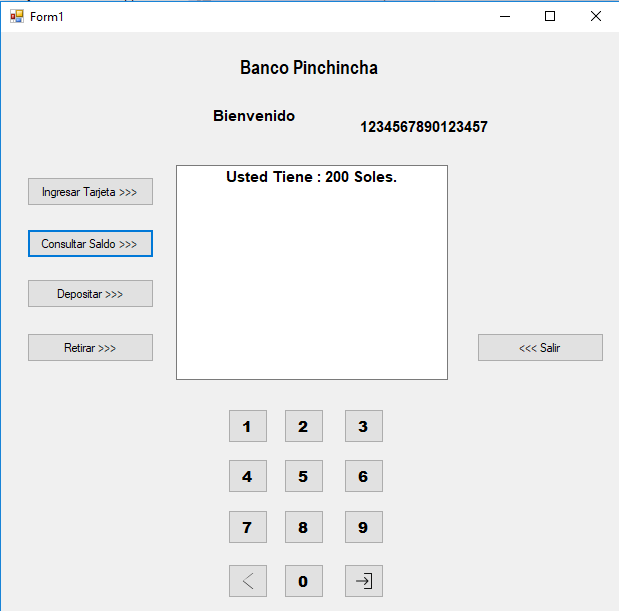
\includegraphics[width=7cm]{./Imagenes/img19}\\

		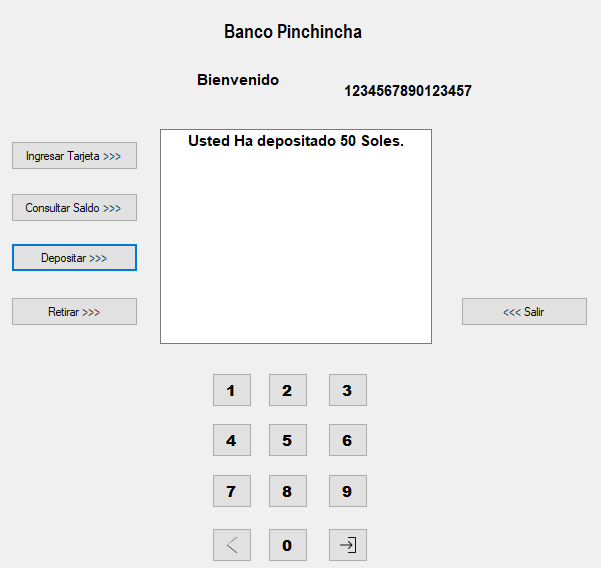
\includegraphics[width=7cm]{./Imagenes/img20}\\

		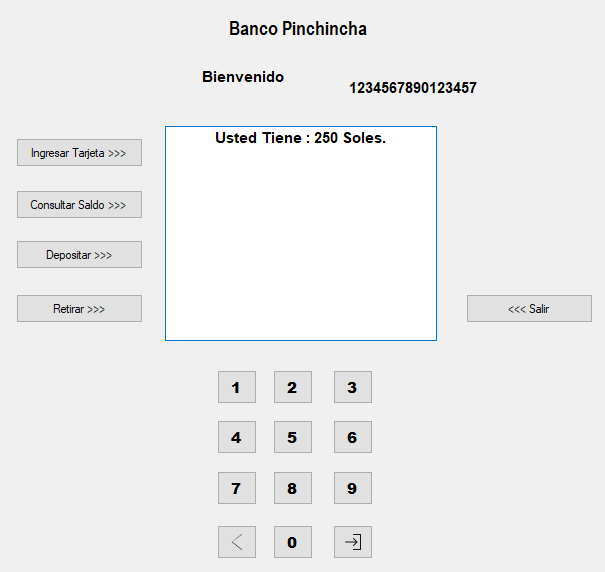
\includegraphics[width=7cm]{./Imagenes/img21}\\

		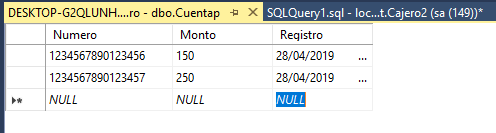
\includegraphics[width=7cm]{./Imagenes/img22}\\

		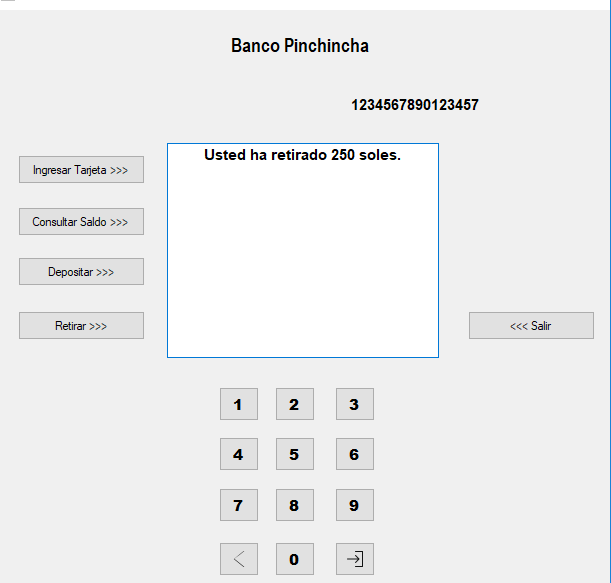
\includegraphics[width=7cm]{./Imagenes/img23}\\

		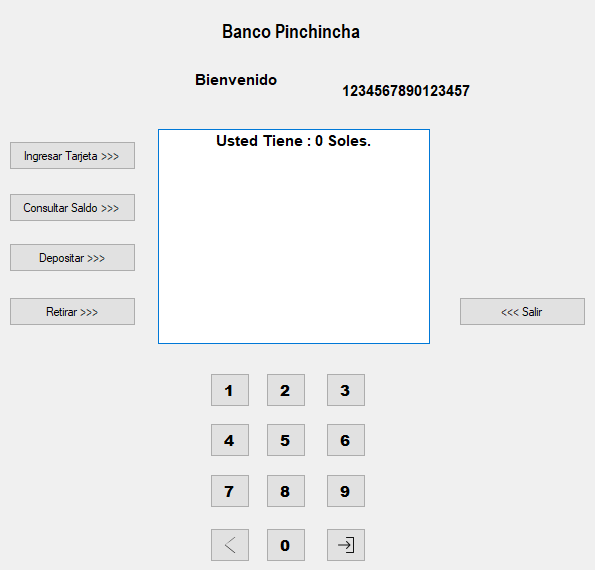
\includegraphics[width=7cm]{./Imagenes/img24}\\
		\end{center}
		\end{figure}
	\item Paso 14: Y así hemos demostradro la funcionalidad con un ORM. Ha quedado demostrado la simplicidad del código que hemos usado.
		\begin{figure}[H]
		\begin{center}
		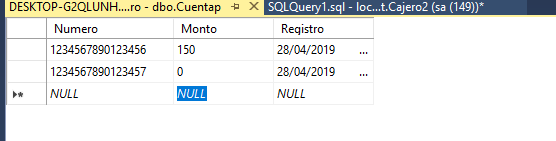
\includegraphics[width=7cm]{./Imagenes/img25}
		\end{center}
		\end{figure}
	\end{enumerate}
\end{enumerate}

\subsection{Analisis}
\begin{enumerate}[1.]
	\item Escribiendo consultas con el operador PIVOT
	\begin{enumerate}[a)]
	\item Analisis de desarrollo del Sistema
		-  Caso de uso del Sistema\\
		\begin{figure}[H]
		\begin{center}
		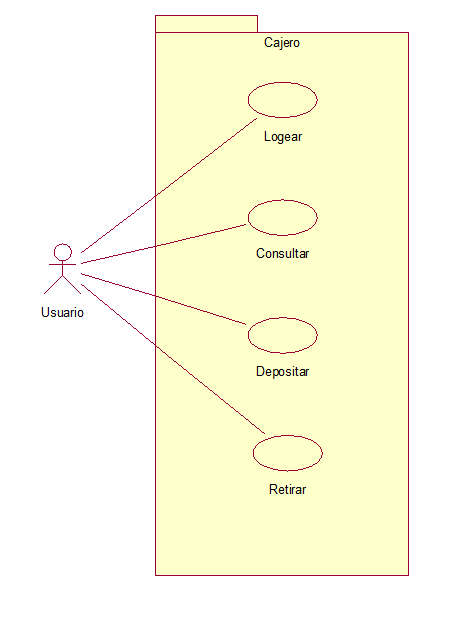
\includegraphics[width=8cm]{./Imagenes/cus}
		\end{center}
		\end{figure}
		-  Diagrama de Entidad Relacion
		\begin{figure}[H]
		\begin{center}
		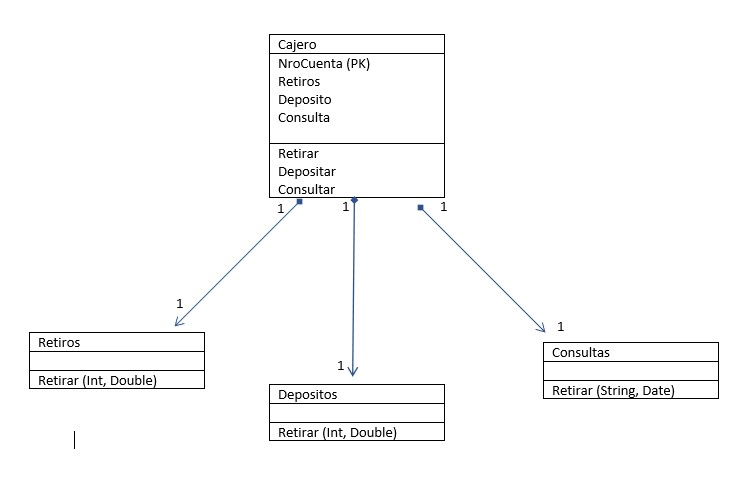
\includegraphics[width=6cm]{./Imagenes/img1}
		\end{center}
		\end{figure}
	\end{enumerate}
\end{enumerate}

	
\subsection{Diseño}
\begin{enumerate}[1.]
	\item Diagrama de Clases, Modelo Entidad Relación
	\begin{enumerate}[a)]
	\item  El diagrama de entidad Relacion fue desarrollado con el fin de que la base de datos tenga una estrutura relacional optima
		\begin{figure}[H]
		\begin{center}
		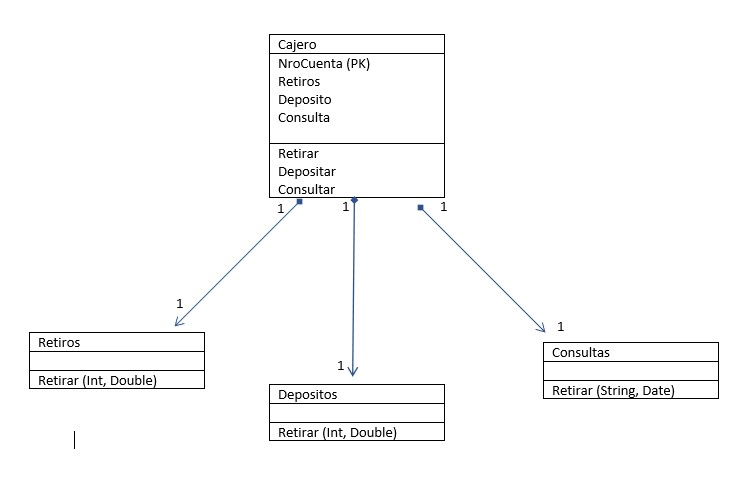
\includegraphics[width=8cm]{./Imagenes/img1}
		\end{center}
		\end{figure}
	\end{enumerate}
\end{enumerate}


\subsection{Pruebas}
\begin{enumerate}[1.]
	\item Pruebas Unitarias
	\begin{enumerate}[a)]
	\item Paso 1: Pruebas unitarias: haremos pruebas unitarias para los métodos deposito, retiro.\\
		-  Agregaremos un test de pruebas unitarias
		\begin{figure}[H]
		\begin{center}
		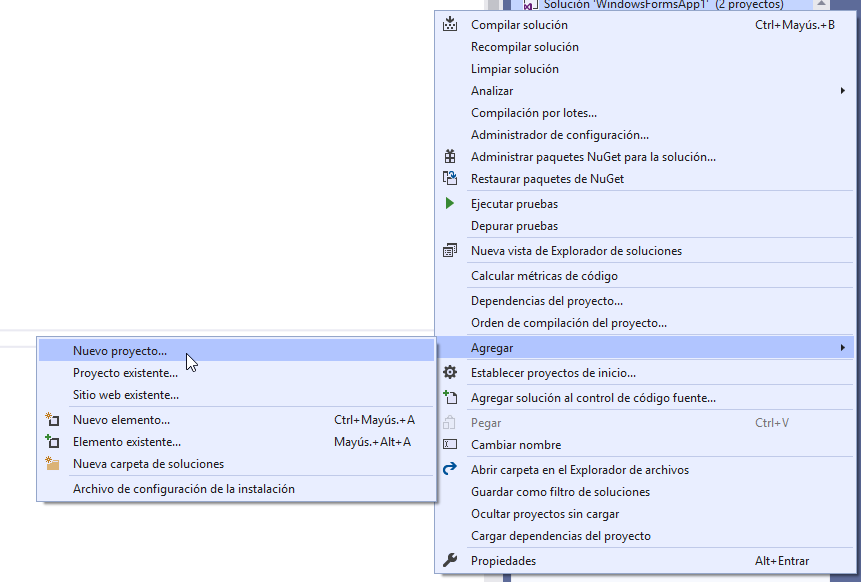
\includegraphics[width=8cm]{./Imagenes/imp1}
		\end{center}
		\end{figure}
	\item Paso 2: Seguidamente el nuevo y tipo de proyecto.
		\begin{figure}[H]
		\begin{center}
		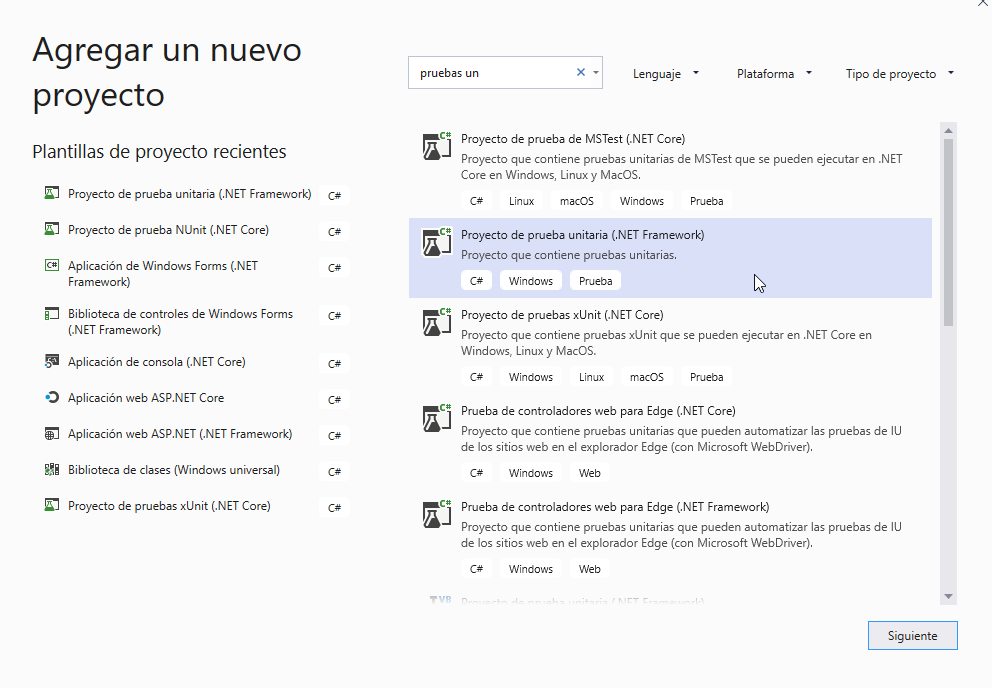
\includegraphics[width=6cm]{./Imagenes/imp2}
		\end{center}
		\end{figure}
	\item Paso 3: Luego referenciaremos el proyecto principal
		\begin{figure}[H]
		\begin{center}
		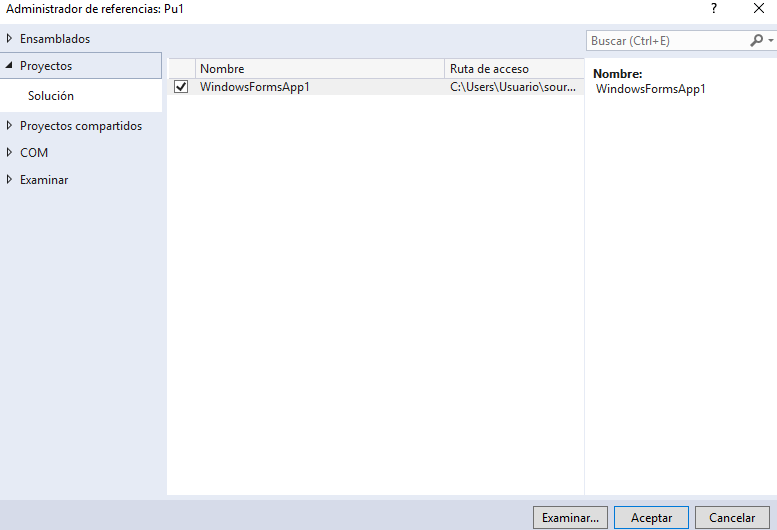
\includegraphics[width=6cm]{./Imagenes/imp3}
		\end{center}
		\end{figure}
	\item Paso 4: Luego probaremos los métodos :
		\begin{figure}[H]
		\begin{center}
		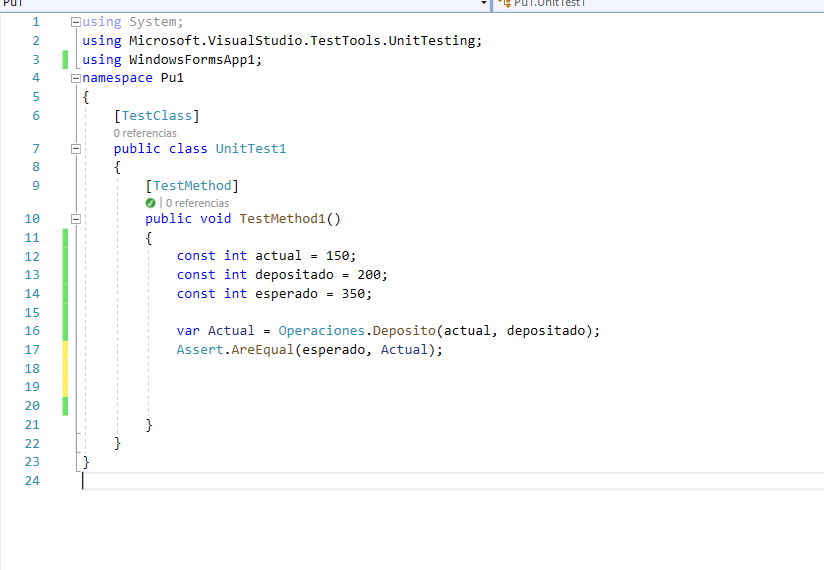
\includegraphics[width=7cm]{./Imagenes/imp4}
		\end{center}
		\end{figure}
	\item Paso 5: Esperamos mientras carga la pruba que se va desarrollar
		\begin{figure}[H]
		\begin{center}
		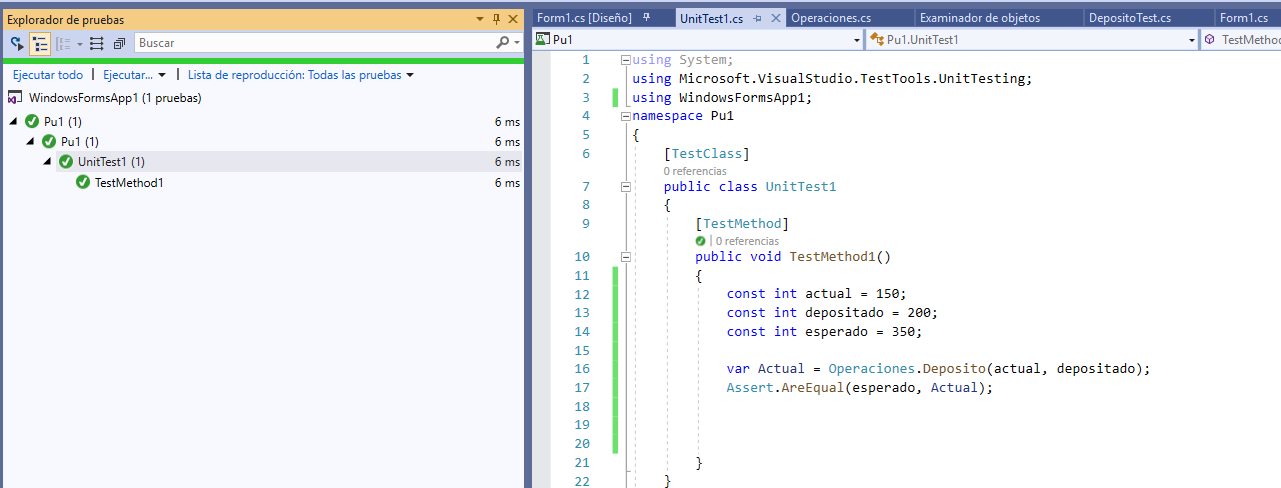
\includegraphics[width=6cm]{./Imagenes/imp5}
		\end{center}
		\end{figure}
	\item Paso 6: Retiros
		\begin{figure}[H]
		\begin{center}
		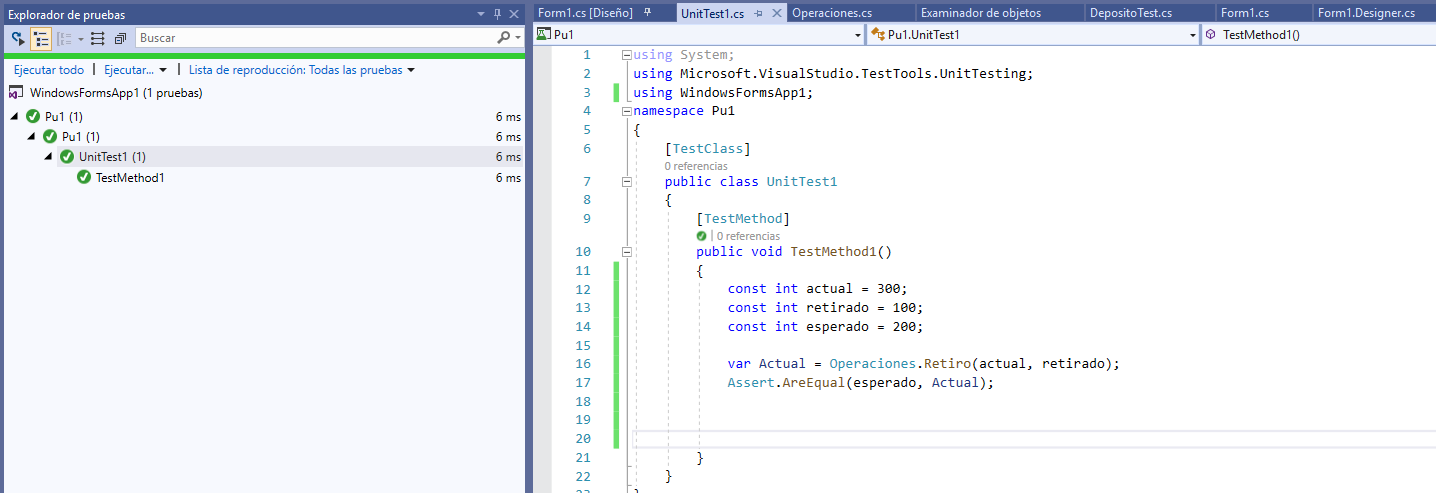
\includegraphics[width=7cm]{./Imagenes/imp6}
		\end{center}
		\end{figure}
	\item Paso 7: Finalmente aplicamos el codigo que se ejecurtar
		\begin{figure}[H]
		\begin{center}
		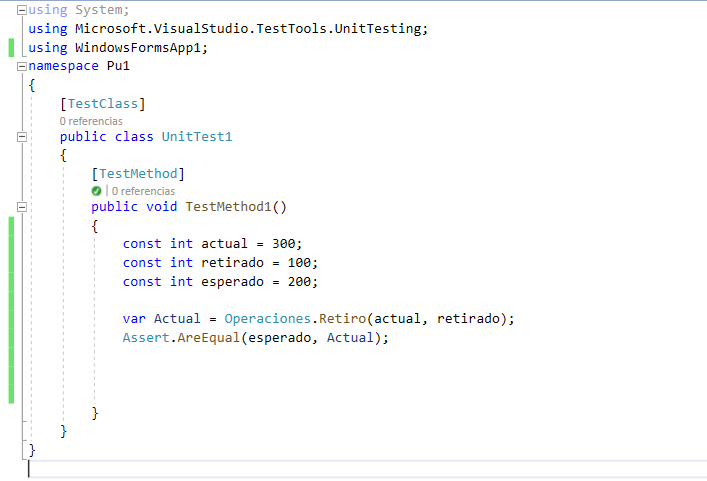
\includegraphics[width=7cm]{./Imagenes/imp7}
		\end{center}
		\end{figure}
	\end{enumerate}
\end{enumerate}





